\documentclass[oneside,a4paper,11pt,explicit]{book}
\usepackage[utf8]{inputenc}
\usepackage{icecream}
\usepackage[english]{babel}
\addto\captionsenglish{\renewcommand{\chaptername}{}}
\usepackage[accsupp]{axessibility}  % improves PDF readability for those with disabilities.
\usepackage[hidelinks,colorlinks = true,urlcolor  = blue]{hyperref}
\usepackage{lipsum}
\usepackage{listings}
\usepackage{minitoc}
\addto{\captionsenglish}{% Making babel aware of special titles
	\renewcommand{\mtctitle}{Quick Links To Sections}
}

\title{I.C.E.C.R.E.A.M. Tutorials}
\subtitle{\small Observing Earth from Above (Env 329) - Fall 2023  \\
	\small Schmid College of Science and Technology Chapman University}
\date{\today}

%% DOCUMENT
\begin{document}
	
\dominitoc

\setcounter{chapter}{3} %Insert (Tutorial Number-1) Here; example for tutorial 4, enter 3

\chapter{Tutorial Name} %Enter Tutorial Name Here

\vspace{-2em}

\minitoc

\section{Section 1}

\kulbox{{\bf Note:} This is an example of a Note Box.}
\lipsum[1]

\section{Figures}
\lipsum[3] 

\vspace{2em}

You can reference figures like this... See Figure: \ref{fig:ECOSTRESS_Logo}.

\vspace{2em}

\lipsum[5] 

\begin{figure}[h]
    \centering
    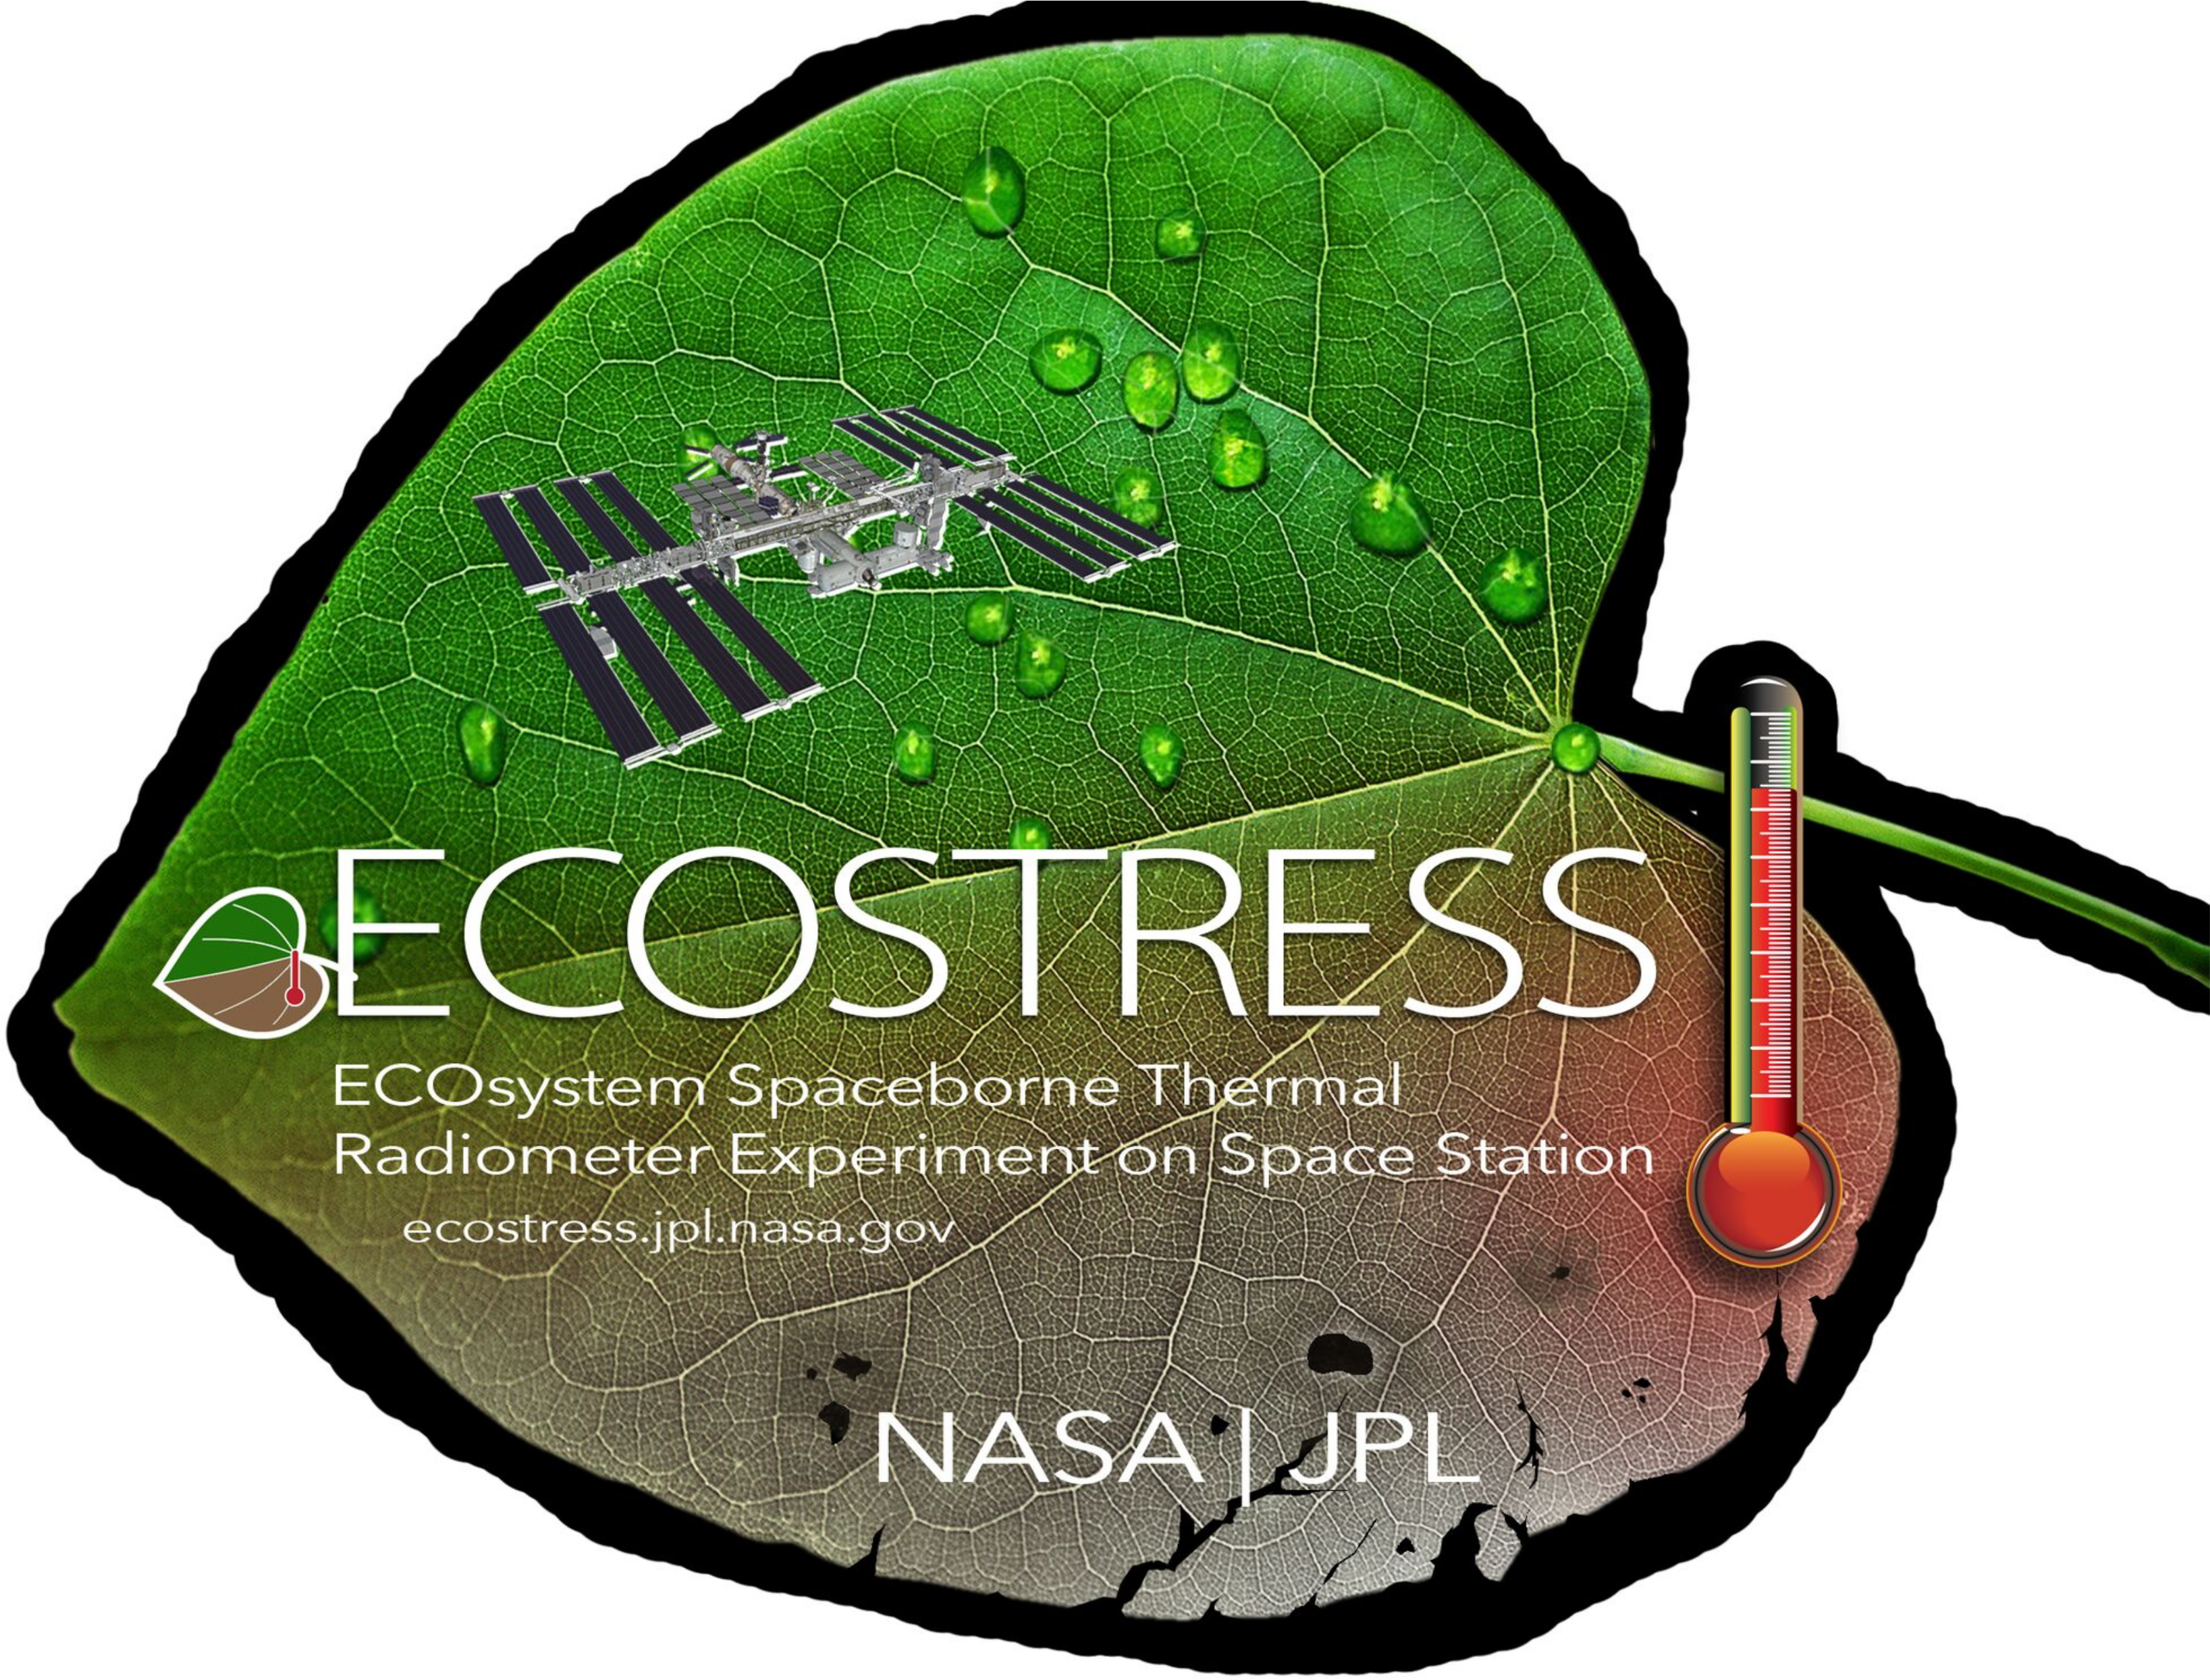
\includegraphics[width=\textwidth]{ECOSTRESS_Logo.png}
    \caption{The ECOSTESS Logo}
    \label{fig:ECOSTRESS_Logo}
\end{figure}

\lipsum[2]

\vfill

\hrule

\vspace{2em}

\textbf{Recommended Citation:} Forsythe, J.D., G.R. Goldsmith, and J.B. Fisher. 2023. Observing Earth from Above Tutorials. Chapman University. \url{https://jeremydforsythe.github.io/icecream-tutorials/}

\vspace{1em}

This work is supported by funding from NASA ECOSTRESS Mission Grant \#80NSSC23K0309 (I.C.E. C.R.E.A.M.: Integrating Communication of ECOSTRESS Into Community Research, Education, Applications, and Media).

\end{document}
